\section{Method}
\label{sec:methods}
In this section, we extend the framework traditionally used to derive Anderson Basis Functions for dipole detection \cite{Otnes2007,https://doi.org/10.1049/rsn2.70091} to the problem of cable detection. \highlight{Rather than adopting the generalized multipolar MOBF formulation of \cite{chenevas2025multipolar}—which will be introduced later in Section \ref{sec:RnD} for comparison—}here we focus on a fundamentally different source: an infinite straight conductor carrying a DC current. To the best of our knowledge, no equivalent OBF have previously been derived for this case.

\subsection{Setup}


Considering the setup shown in Figure \ref{fig:sensor_traj}. A sensor moves at a constant speed $v$ at a fixed altitude $d$ above an infinitely long straight cable carrying a DC current $I$. The system is described in a CPA frame of reference, whose origin is located at the closest point of approach (CPA) and which is rotated by an angle $\psi$ relative to the magnetic north. The sensor crosses the cable at an angle $\theta$.

\begin{figure}[h]
\centering
\begin{minipage}{0.48\linewidth}
    \centering
    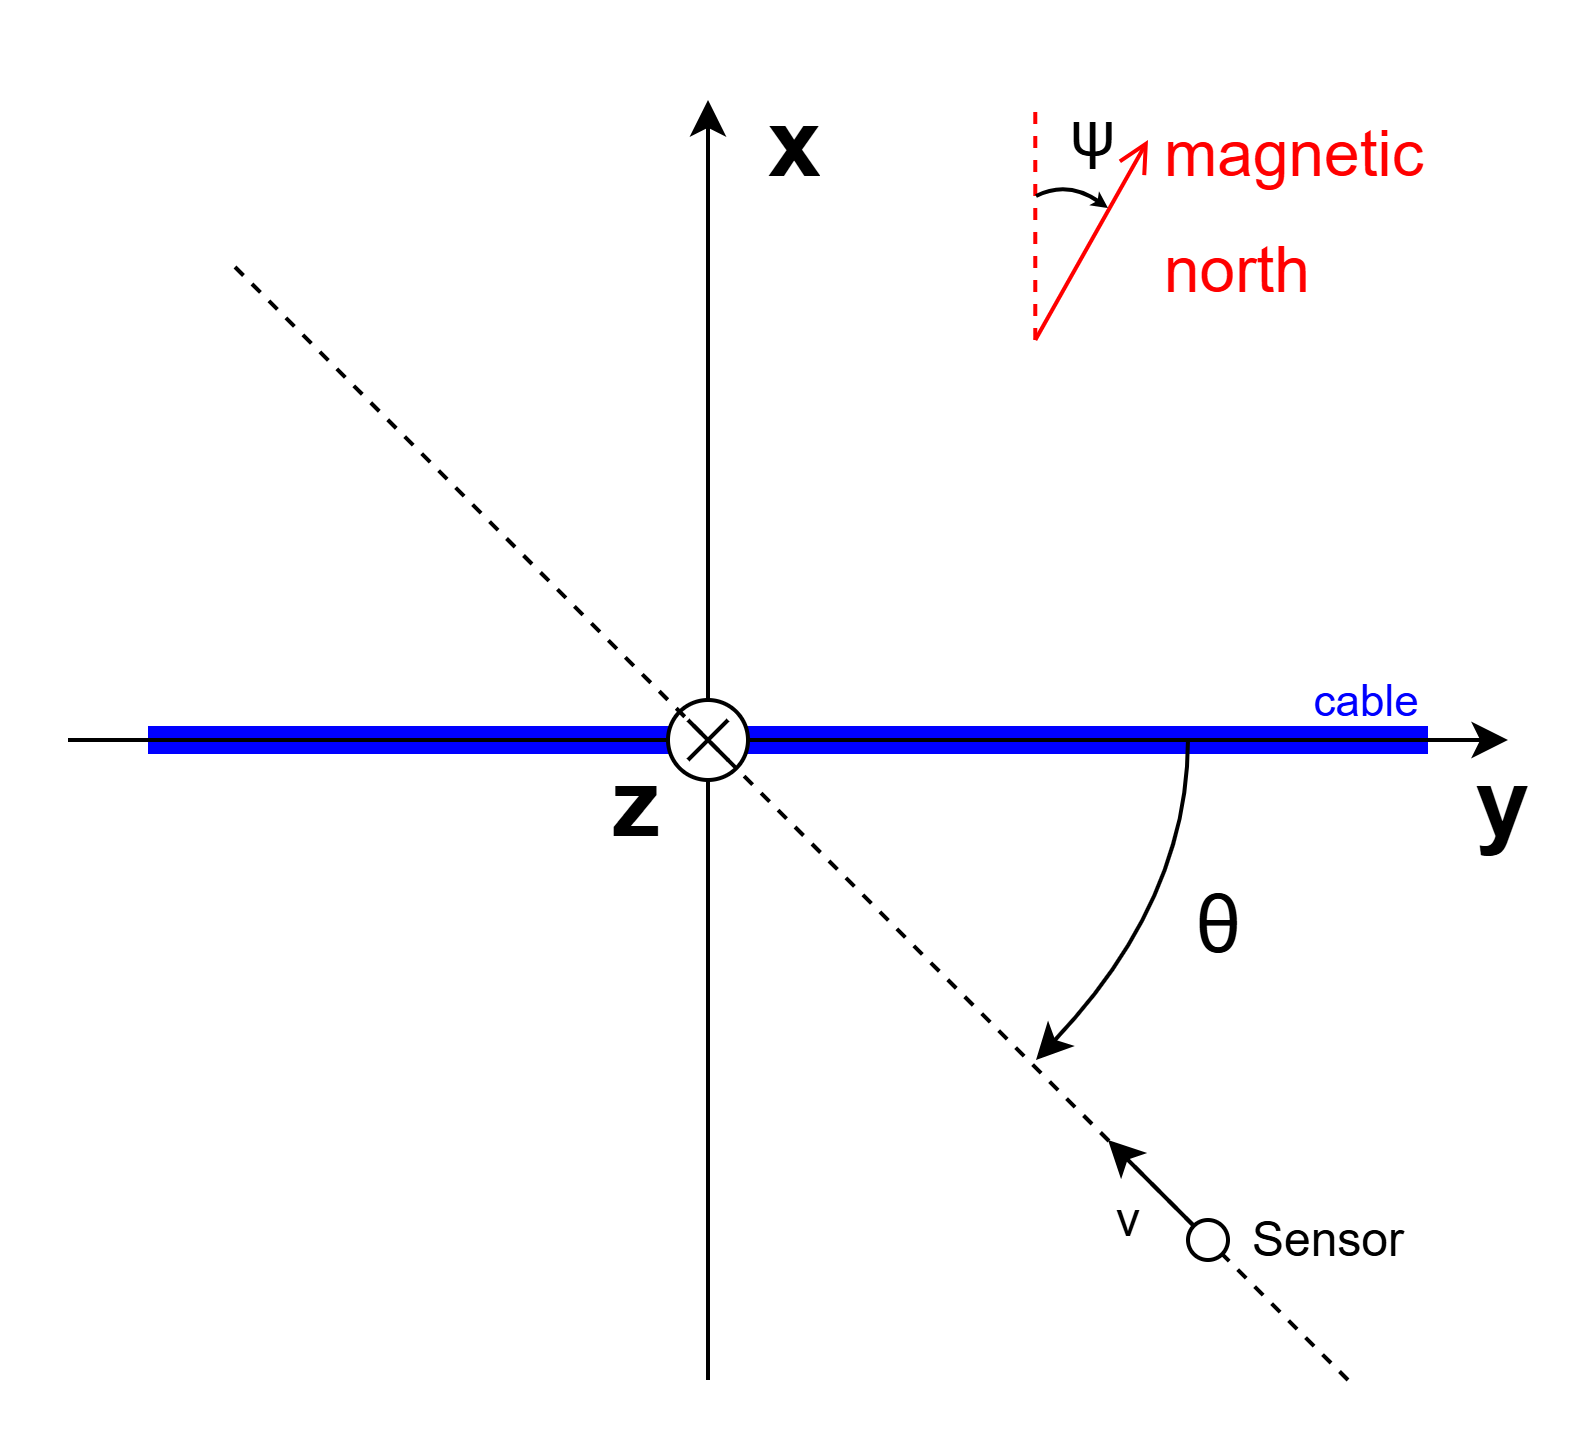
\includegraphics[width=\linewidth]{methodology/figures/sensor_trajectory1.png}
\end{minipage}
\hfill
\begin{minipage}{0.48\linewidth}
    \centering
    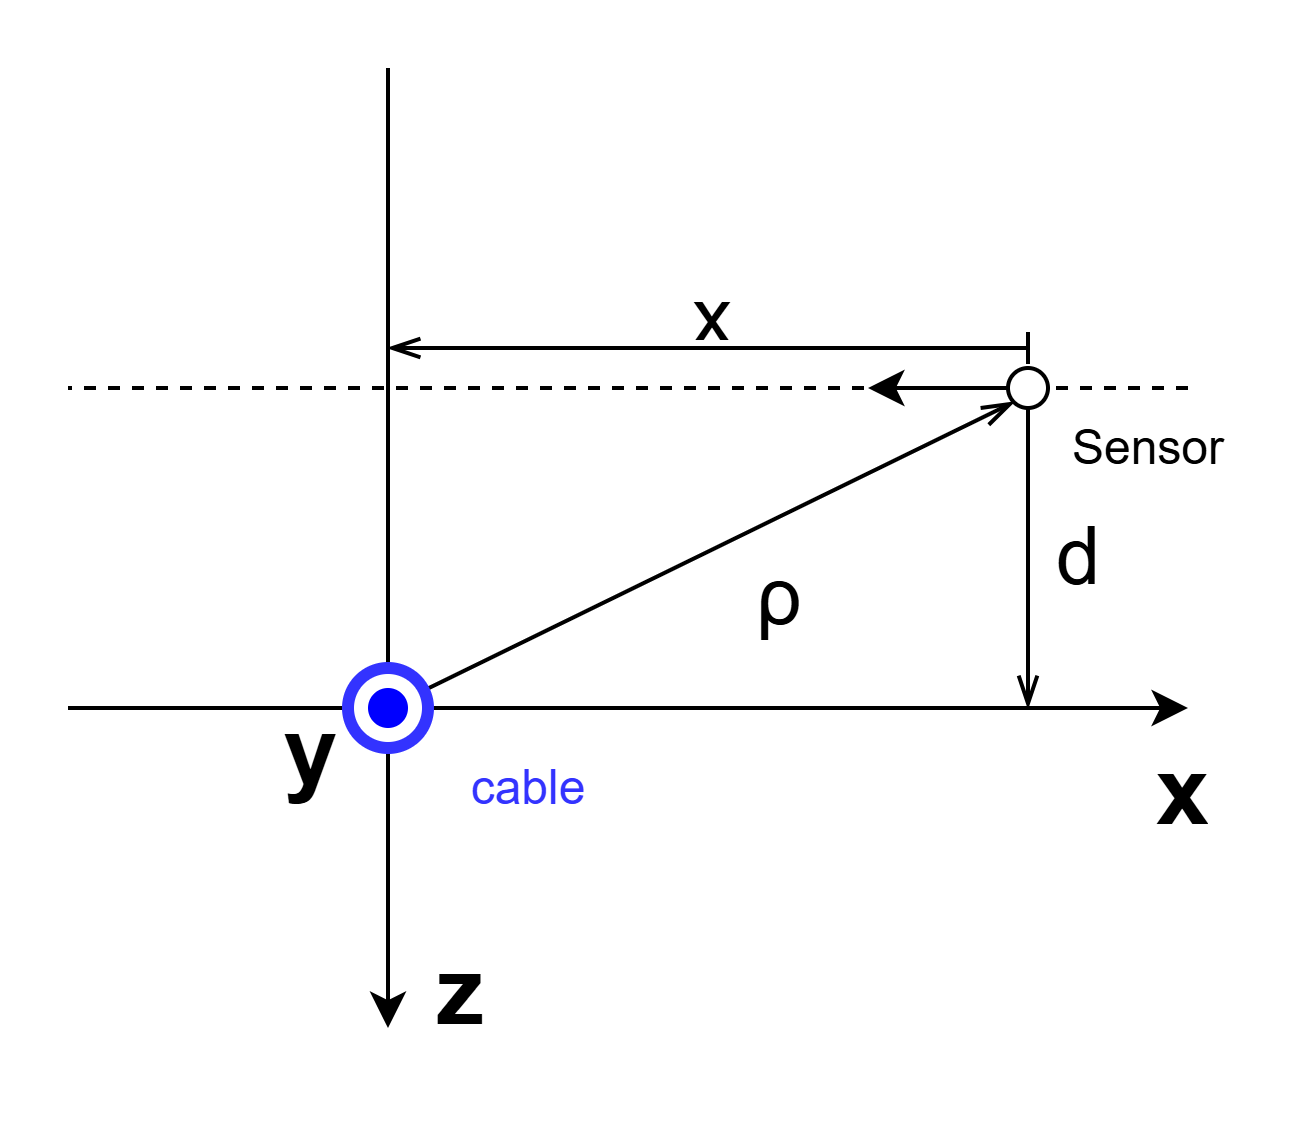
\includegraphics[width=\linewidth]{methodology/figures/sensor_trajectory2.png}
\end{minipage}
    \caption{Sensor trajectory in the CPA frame of reference, on the left (top down view), on the right (profile view)}
    \label{fig:sensor_traj}
\end{figure}

\highlight{Starting from the expression of the magnetic field in the CPA frame of reference, and noting that, as an underwater telecommunications cable, the return current is via the seawater, which motivates modeling the cable as an infinite straight conductor carrying current in a single direction, under this assumption, the magnetic field is obtained using the classical Biot–Savart law:}

\begin{equation*}
    \vec{B} = \frac{\mu_0}{4\pi} \int \frac{I \, d\vec{\ell} \times \hat{r}}{r^2}
\end{equation*}

where, in our application, \(d\vec{\ell}\) is \(d\vec{y}\), and \(\vec{r}\) is \(\vec{\rho}\)   (the radial sensor position relative to the cable), further development will give :
\highlight{
\begin{equation}
    \vec{B} = \frac{\mu_0 I}{2\pi \rho}\,\vec{e}_{az}
    \label{eq:mag_field}
\end{equation}

where $\vec{e}_{az}$ is the azimuthal unit vector (right-hand rule).

\begin{equation*}
\vec{e}_{az} = \frac{d\vec{y} \times \vec{\rho}}{\rho}
= \frac{1}{\rho}
\begin{pmatrix}
0 \\ 1 \\ 0
\end{pmatrix}
\times
\begin{pmatrix}
-x \\ 0 \\ d
\end{pmatrix}
=  \frac{1}{\rho}
\begin{pmatrix}
d \\ 0 \\ x
\end{pmatrix}
\end{equation*}
}
Although \(\vec{B}\) is inherently a spatial field, the sensor motion causes it to be observed as a time-varying signal \(\vec{B}_s(t) = \vec{B}(\mathbf{\rho}(t))\).

Assuming a rectilinear trajectory, the sensor position along the \(x\)-axis is given by
\(
x(t) = v t \sin(\theta)
\)
and $\rho(t) = \sqrt{x^2(t) + d^2}$.

For simplicity, we assume that the sensor does not rotate, \textit{i.e., its local \(x\) and \(z\) axes remain aligned with those of the CPA frame at all times}.

The measured magnetic field in the sensor frame is then
\begin{equation*}
    \vec{B}_s(t) =  \frac{\mu_0 I}{2 \pi} 
    \begin{pmatrix}
        \dfrac{d}{\rho^2(t)} \\[6pt]
        0 \\[6pt]
        \dfrac{x(t)}{\rho^2(t)}
    \end{pmatrix},
\end{equation*}

This expression can be normalized with respect to time, velocity, and trajectory angle \(\theta\) by introducing the dimensionless variable
\[
\tau = \frac{x(t)}{d} = \frac{v t \sin(\theta)}{d}.
\]

After simple factorization, the normalized magnetic field measurement becomes
\begin{equation*}
    \vec{B}_s(\tau) = \frac{\mu_0 I}{2 \pi d}
    \begin{pmatrix}
        \dfrac{1}{1+\tau^2} \\[6pt]
        0 \\[6pt]
        \dfrac{\tau}{1+\tau^2}
    \end{pmatrix}.
\end{equation*}

\subsection{Magnetic Anomaly Approximation}
In reality, the Earth's magnetic field \(\Vec{T}\) is always present, and if we assume that there are no sources for magnetic anomalies other than the cable, the sensor records:
\begin{equation*}
    \vec{F_s} = \vec{T} + \vec{B}_s
\end{equation*}

Moreover, in practical situations one typically has \(\vec{B}_s << \vec{T}\), with \(B_s\) on the order of \(\mu\text{T}\). Consequently, \highlight{for a scalar magnetometer \footnote{Practically, the norm of a fluxgate magnetometer is used, for its lower cost, and taking its norm makes it more robust against the noise from trajectory fluctuations and other types of external motion noise.} recording \(F_s\), \(B_s\) can be treated as the projection of \(\vec{B}_s\) onto the unitary vector of the Earth's magnetic field \(\vec{T}\), which is constant during measurements, \cite[Chapter~2, Section~7.2]{nodot:tel-01155714}, see Figure~\ref{fig:ill_anom}.}

\begin{figure}
    \centering
    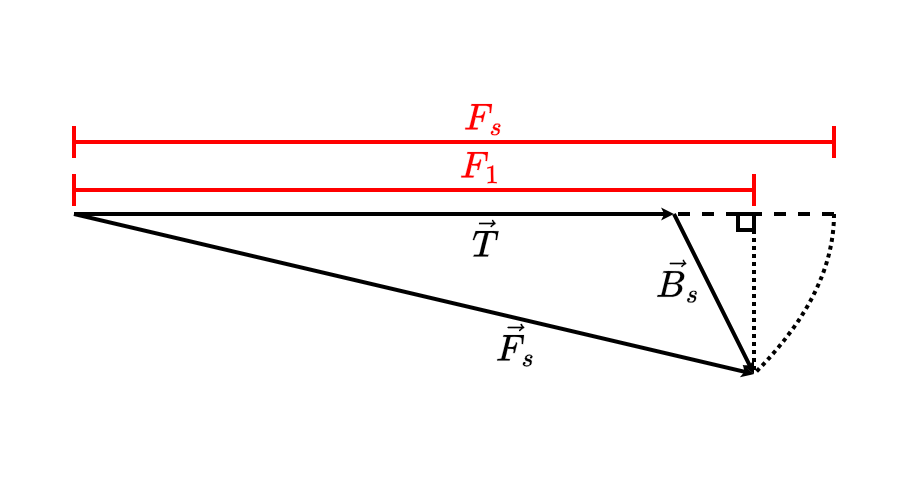
\includegraphics[width=\linewidth]{methodology/figures/anomaly_geometry.png}
    \caption{geometrical illustration of the magnetic anomaly}
    \label{fig:ill_anom}
\end{figure}

thus,
\begin{equation*}
    \lvert \vec{F_s} \lvert \approx F_1 = \lvert\vec{T}\lvert + \frac{\vec{B_s}.\vec{T}}{\lvert\vec{T}\lvert}
\end{equation*}
The magnetic anomaly generated by the cable is approximately:
\begin{equation*}
    S \approx F_1 - \lvert\vec{T}\lvert = \frac{\vec{B_s}.\vec{T}}{\lvert\vec{T}\lvert}
\end{equation*}

To generalize the model, Earth's magnetic field is inclined by \(\delta\), and the CPA reference axis forms an angle \(\psi\) with magnetic north:
{\scriptsize
\begin{equation*}
    S(\tau) = \frac{\mu_0 I}{2 \pi d} 
    \left(
    \begin{pmatrix}
        \cos{\psi} & -\sin{\psi} & 0 \\
        \sin{\psi} & \cos\psi & 0 \\
        0 & 0 & 1
    \end{pmatrix}
    \begin{pmatrix}
        \frac{1}{1+\tau^2} \\ 0 \\ \frac{\tau}{1+\tau^2}
    \end{pmatrix}
    \right)
    \cdot
    \begin{pmatrix}
        \cos\delta \\ 0 \\ \sin\delta
    \end{pmatrix}
\end{equation*}
}

Developing and refactoring the previous equation gives:

\begin{equation}
\begin{aligned}
S(\tau) &= K_p \cdot \cos\psi \cdot \cos\delta \cdot \frac{1}{1+\tau^2} 
        + K_p \cdot \sin\delta \cdot \frac{\tau}{1+\tau^2} \\
K_p &=  \frac{\mu_0 I}{2 \pi d}.
\end{aligned}
\label{eq:anomaly}
\end{equation}

\subsection{Derivation of Cable OBF}\label{sec:signal_representation}
To construct a detector, we decompose the signal into orthonormal components, \(S(\tau)\) can be written as \(S(\tau) = \sum_{n=1}^{2} a_n\, f_n(\tau).\)
where \(f_n(\tau\)) are the only terms that depend on time.
\begin{equation*}
    S(\tau) = \underbrace{K_p \cdot\cos\psi \cdot \cos\delta }_{{a_1}}                
              \underbrace{\frac{1}{1+\tau^2}}_{{f_1(\tau)}}
              +
              \underbrace{K_p \cdot\sin\delta}_{{a_2}}              
              \underbrace{\frac{\tau}{1+\tau^2}}_{{f_2(\tau)}}
\end{equation*}

Similar to the Anderson functions for dipoles, we can propose \(f_1(\tau)\) and \(f_2(\tau)\) as basis functions for cables, they just need to be orthonormalized, satisfying the following criteria:

\begin{equation*}
    \int_{-\infty}^{+\infty} \Phi_i(\tau)\, \Phi_j(\tau)\, d\tau = \delta_{ij}
\end{equation*}

where $\delta_{ij}$ is the Kronecker delta:

\[
    \delta_{ij} =
    \begin{cases}
        1 & \text{if } i = j \\
        0 & \text{if } i \neq j
    \end{cases}
\]
As the functions are already orthogonal, it is sufficient to normalize them, thus, we assume:
\begin{equation*}
    \Phi_1 = \kappa_1 f_1, \qquad \Phi_2 = \kappa_2 f_2
\end{equation*}
Solving for the normalization constants yields:

\begin{equation*}
    \kappa_1 = \kappa_2 = \sqrt{\frac{2}{\pi}}
\end{equation*}

The orthonormal basis functions for a cable carrying a DC current are therefore given by
\begin{equation}
    \Phi_1(\tau) = \sqrt{\frac{2}{\pi}}\,\frac{1}{1+\tau^2}, \qquad
    \Phi_2(\tau) = \sqrt{\frac{2}{\pi}}\,\frac{\tau}{1+\tau^2},
    \label{eq:OBF}
\end{equation}
where the normalized time parameter is defined as \(\tau = \frac{v\sin\theta}{d}\,t\).

\highlight{These OBF are plotted in Figure~\ref{fig:basis_funs} alongside MOBF from \cite{chenevas2025multipolar}, for order 1, which are the well-known Anderson functions for dipoles, and order 2, which combines the basis functions of a dipole and a quadrupole.}

Finally substituting equation~\eqref{eq:OBF} into the expression for the magnetic anomaly in equation~\ref{eq:anomaly},
yields the final anomaly signal representation for detection:
\begin{equation}
    S(\tau) = A_1\Phi_1(\tau) + A_2\Phi_2(\tau),
    \label{eq:anomaly_final}
\end{equation}
where \(A_1\) and \(A_2\) are the OBF amplitudes determined by the current, cable depth and orientation.

\begin{figure*}[t]
    \centering
    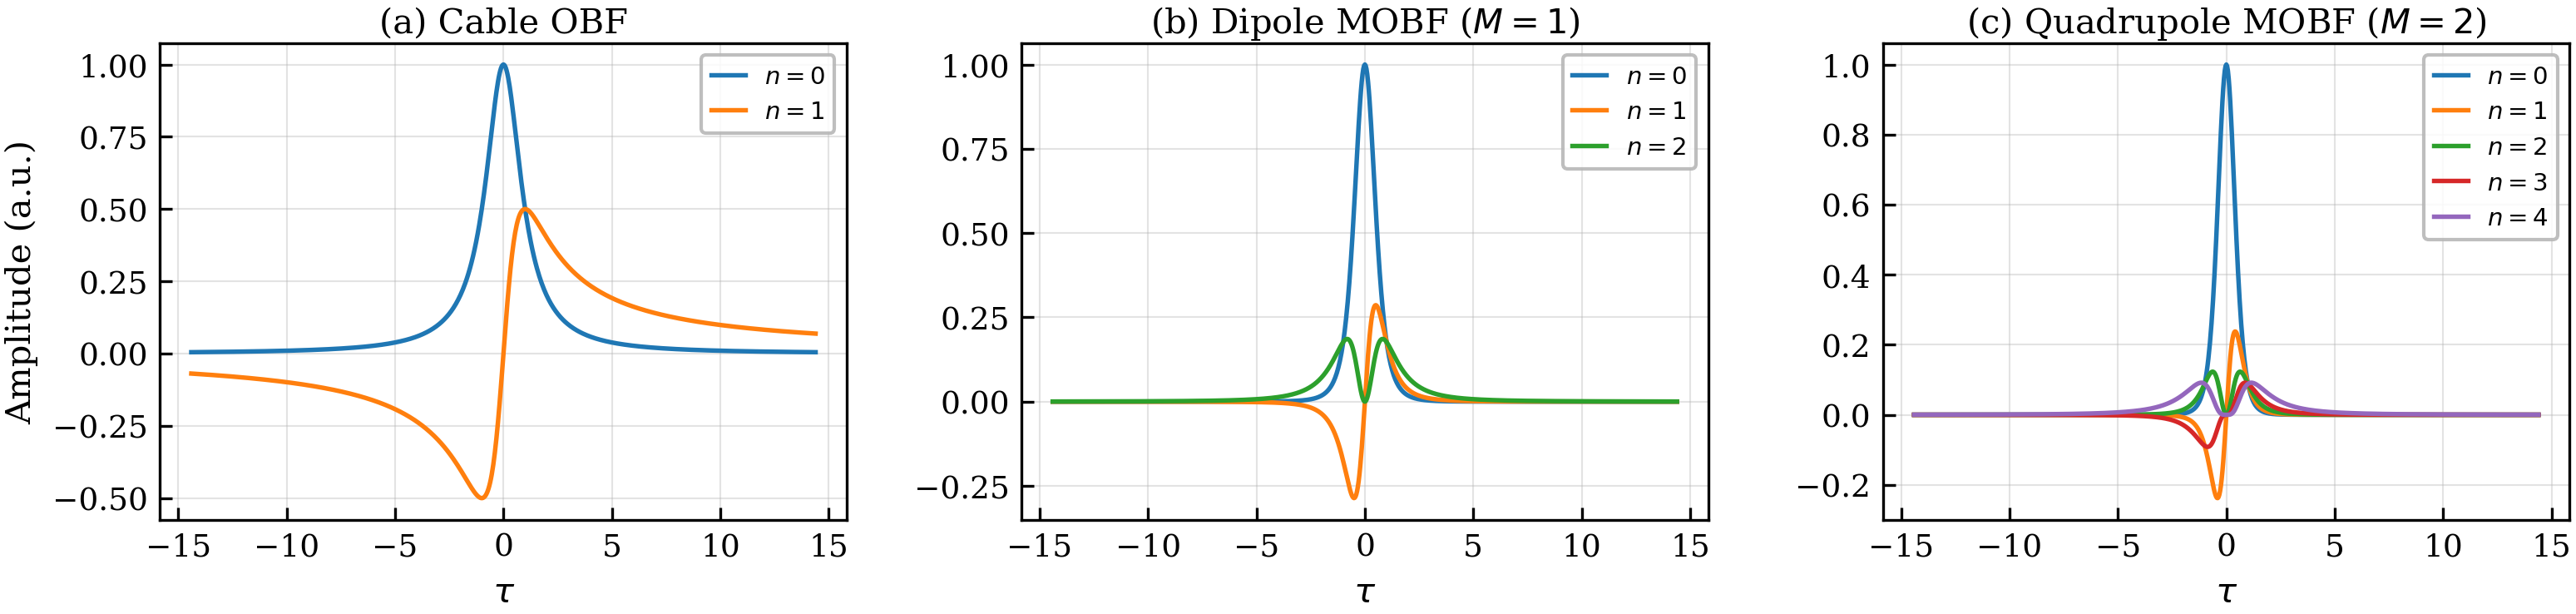
\includegraphics[width=\textwidth]{results_and_discus/figures/basis_functions_multipole.png}
    \caption{Basis functions for dipole and cable.}
    \label{fig:basis_funs}
\end{figure*}


\subsection{Generalized Matched Filter Detector}
\label{sec:detector}

Model-based magnetic anomaly detection showed a robustness for dipole detection \cite{https://doi.org/10.1049/rsn2.70091}. Those detection problems are usually formulated as the detection of known signals with unknown amplitudes embedded in noise, assuming an additive white Gaussian noise (AWGN). The optimal solution to this kind of problem becomes a Generalized matched filter (GMF) combined with a Generalized likelihood ratio test (GLRT) \cite{Kay1998Detection}.

The orthogonality of the chosen basis functions ensures that the signal components are uncorrelated. This property significantly simplifies the GMF structure by reducing it to two independent matched filters, one for each basis function. Under these conditions, and regarding equation~\eqref{eq:anomaly_final} the GLRT can be formulated with the following hypotheses:
\begin{align*}
\mathcal{H}_0 &: X(\tau) = w(\tau)\\
\mathcal{H}_1 &: X(\tau) = A_1 \Phi_1(\tau) + A_2 \Phi_2(\tau) + w(\tau)
\end{align*}
where \(A_1\) and \(A_2\) are the unknown signal amplitudes, \(\Phi_1(\tau)\) and \(\Phi_2(\tau)\) are the orthonormal basis functions and the signal templates for the matched filters, and \(w(\tau) \sim \mathcal{N}(0, \sigma^2)\) represents the noise.


We note that in practice, we de-normalize the basis functions (so they become a function of time $t$), reducing the calculation needed to normalize the input signal $X(t)$. The corresponding detection procedure and statistical characterization are illustrated in Figure~\ref{fig:filter_diagram}.
\begin{figure}
    \centering
    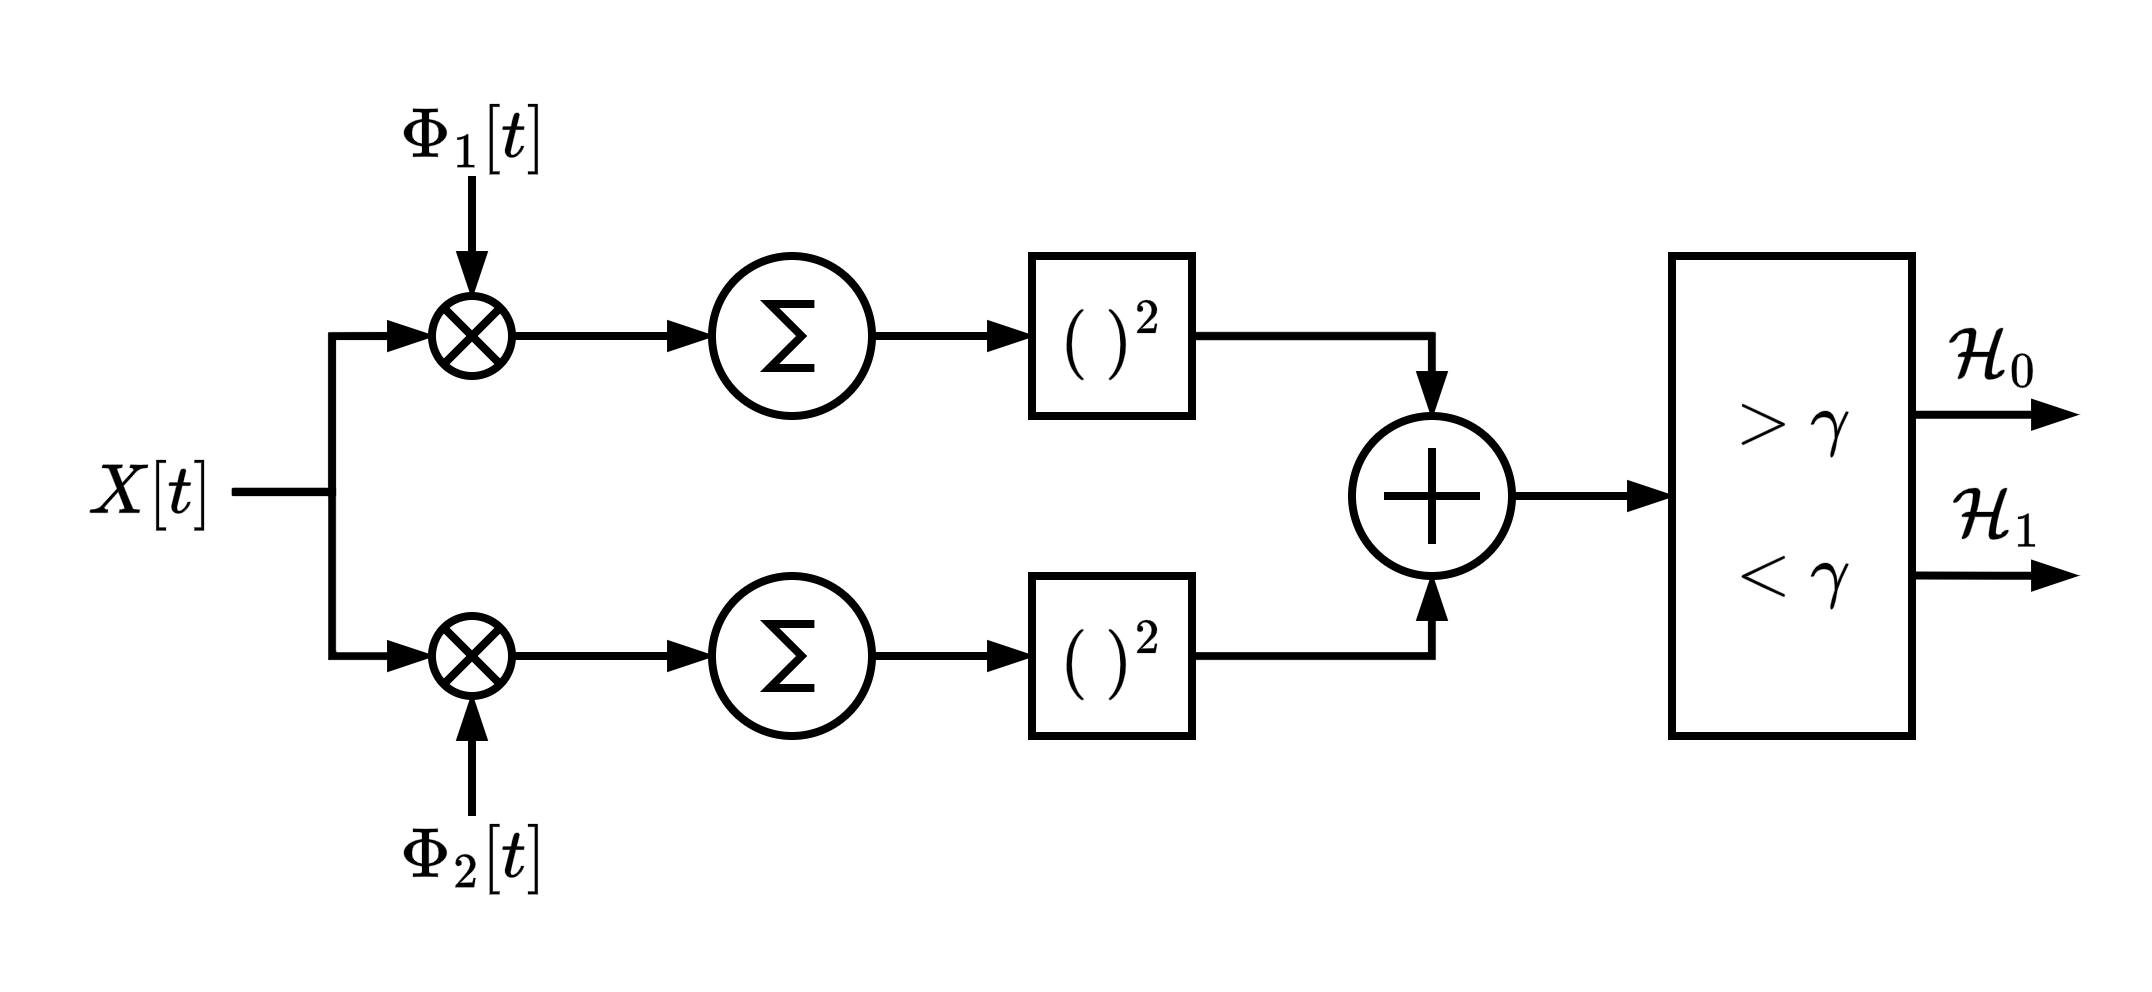
\includegraphics[width=1\linewidth]{methodology//figures/filter_diagram.png}
    \caption{diagram of the matched filter and hypothesis test used for magnetic anomaly detection}
    \label{fig:filter_diagram}
\end{figure}

\highlight{In the remainder of this work, experiments were conducted to determine under which conditions the proposed cable OBF method outperforms the established MOBF approach for the task of cable detection.}